% ============================================================================
%  RIGEL — CSE 220 Signals and Linear Systems Sessional — Project Presentation
%  Team Orion
% ============================================================================
\documentclass[11pt,aspectratio=169]{beamer}

\usepackage{fontspec}
\usepackage{soul}
\usepackage{tikz}
\usetikzlibrary{shadings,fadings,positioning,arrows.meta,calc}
\usepackage{amsmath,amssymb}
\usepackage{graphicx}
\usepackage{xcolor}
\usepackage[absolute,overlay]{textpos}

\setmainfont{segoeui.ttf}[
  BoldFont = seguisb.ttf,
  ItalicFont = segoeuii.ttf,
  BoldItalicFont = seguisbi.ttf
]
\setsansfont{segoeui.ttf}[
  BoldFont = seguisb.ttf,
  ItalicFont = segoeuii.ttf,
  BoldItalicFont = seguisbi.ttf
]
\setmonofont{TeX Gyre Cursor}
\renewcommand{\familydefault}{\sfdefault}

% Rivage font from uploaded Rivage.ttf
\newfontfamily\rivagefont{Rivage.ttf}

% ---------------------------------------------------------------------------
% Colour palette — matches frontend/src/app/globals.css design tokens
% ---------------------------------------------------------------------------
\definecolor{rigelBg}{RGB}{8,8,17}
\definecolor{rigelCard}{RGB}{13,13,23}
\definecolor{rigelCard2}{RGB}{18,18,30}
\definecolor{rigelBorder}{RGB}{42,42,60}
\definecolor{rigelFg}{RGB}{255,255,255}
\definecolor{rigelMuted}{RGB}{148,163,184}
\definecolor{rigelMuted2}{RGB}{100,116,139}
\definecolor{rigelPrimary}{RGB}{79,70,229}
\definecolor{rigelAccent}{RGB}{129,140,248}
\definecolor{rigelAccentLight}{RGB}{180,190,253}
\definecolor{rigelCyan}{RGB}{34,211,238}
\definecolor{rigelGreen}{RGB}{52,211,153}
\definecolor{rigelGlow1}{RGB}{67,56,180}
\definecolor{rigelGlow2}{RGB}{30,58,138}

\setbeamercolor{background canvas}{bg=rigelBg}
\setbeamercolor{normal text}{fg=rigelFg,bg=rigelBg}
\setbeamercolor{itemize item}{fg=rigelAccent}
\setbeamercolor{itemize subitem}{fg=rigelMuted}
\setbeamertemplate{navigation symbols}{}
\setbeamertemplate{itemize item}{\textcolor{rigelAccent}{\rule{1.6mm}{1.6mm}}}
\setbeamertemplate{itemize subitem}{\textcolor{rigelMuted2}{\rule{1.1mm}{1.1mm}}}
\setlength{\parskip}{4pt}
\setlength{\parindent}{0pt}
\setbeamersize{text margin left=10mm,text margin right=10mm}

% ---------------------------------------------------------------------------
% Background: deep navy canvas + soft indigo glows + faint starfield
% ---------------------------------------------------------------------------
\setbeamertemplate{background}{%
  
\begin{tikzpicture}[remember picture]
    \fill[rigelBg] (0,0) rectangle (16cm,9cm);
    \shade[shading=radial,inner color=rigelGlow1,outer color=rigelBg,opacity=0.32]
      (13.75cm,8.25cm) circle (4.25cm);
    \shade[shading=radial,inner color=rigelGlow2,outer color=rigelBg,opacity=0.30]
      (0.75cm,0.5cm) circle (3.5cm);
    \foreach \x/\y in {0.05/0.88,0.14/0.22,0.31/0.93,0.46/0.10,0.58/0.78,
                       0.69/0.30,0.79/0.90,0.89/0.15,0.94/0.58,0.23/0.52,
                       0.40/0.38,0.63/0.06,0.03/0.45,0.97/0.80}
      {\fill[white,opacity=0.28] ({\x*16cm},{\y*9cm}) circle (0.4pt);}
  \end{tikzpicture}%
}

% ---------------------------------------------------------------------------
% Professional Executive Footer
% ---------------------------------------------------------------------------
\setbeamertemplate{footline}{%
  \leavevmode%
  \begin{tikzpicture}[remember picture, overlay]
    % Subtle top separator rule across slide width with margin padding
    \draw[color=rigelBorder, line width=0.45pt] 
      ($(current page.south west) + (0.9cm, 0.65cm)$) -- 
      ($(current page.south east) + (-0.9cm, 0.65cm)$);
  \end{tikzpicture}%
  \hbox{%
    \begin{beamercolorbox}[wd=\paperwidth,ht=3.8ex,dp=2.2ex,leftskip=0.9cm,rightskip=0.9cm]{footline}%
      % Left: Project & Affiliation
      {\fontsize{6.8}{8}\selectfont%
        \textcolor{rigelAccent}{\raisebox{-0.5pt}{\fontsize{8.5}{8.5}\selectfont\rivagefont Rigel}}%
        \hspace{0.55em}\textcolor{rigelBorder}{|}\hspace{0.55em}%
        \textcolor{rigelMuted}{Team Orion}%
      }%
      \hfill%
      % Center: Contextual section name (if set)
      {\fontsize{6.5}{8}\selectfont\color{rigelMuted2}%
        \ifx\insertsection\empty\else\insertsection\fi%
      }%
      \hfill%
      % Right: Sleek slide counter pill
      \tikz[baseline=-0.5ex]{%
        \node[rounded corners=3pt, fill=rigelCard2, draw=rigelBorder, 
              line width=0.4pt, inner sep=2.5pt, inner xsep=5pt] {%
          \fontsize{6.5}{6.5}\selectfont\ttfamily\color{rigelFg}%
          \insertframenumber\,\textcolor{rigelMuted2}{/}\,\inserttotalframenumber%
        };%
      }%
    \end{beamercolorbox}%
  }%
}

% ---------------------------------------------------------------------------
% Header block: small tracked kicker + big title + accent underline
% ---------------------------------------------------------------------------
% Word space increased from 0.3em -> 0.55em so words don't collide
\sodef\rigeltrack{}{0.16em}{0.65em plus0.15em}{0.4em plus0.15em minus0.05em}

\newcommand{\rigelheader}[2]{%
  \vspace{0.5mm}
  {\fontsize{8}{8}\selectfont\bfseries\color{rigelAccent} #1}\\[3pt]
  {\fontsize{18.5}{19.5}\selectfont\bfseries\color{rigelFg} #2}\\[2pt]
  {\color{rigelPrimary}\rule{1.8cm}{1.4pt}}
  \vspace{4.0mm} % Increased from 1.5mm -> 4.0mm for breathing room before content
}

% ---------------------------------------------------------------------------
% Screenshot card macro — enlarged & auto-fitted across all slides
% ---------------------------------------------------------------------------
\newcommand{\rigelshot}[2][]{%
  \begin{center}
  \vspace{-2mm}% Pulls the card slightly higher into available top space
  \begin{tikzpicture}
    \node[rounded corners=4pt, draw=rigelBorder, line width=0.8pt,
          fill=rigelCard, inner sep=4pt]
      {\scalebox{1.22}{\includegraphics[#1,max width=0.82\linewidth,max height=4.9cm,keepaspectratio]{#2}}};
  \end{tikzpicture}
  \end{center}
  \vspace{-1.5mm}% Tightens space beneath the card so bullet points fit comfortably
}

% ---------------------------------------------------------------------------
% Small planet logomark (vector, reused on title / closing slides)
% ---------------------------------------------------------------------------
\newcommand{\rigelplanet}[1][1.0]{%
  \begin{tikzpicture}
    \shade[shading=radial,inner color=rigelCyan!70!white,
           outer color=rigelPrimary!70!black] (0,0) circle (#1);
    \draw[rigelAccentLight,opacity=0.55,line width=0.5pt]
      (0,0) ellipse ({#1*1.55} and {#1*0.55});
  \end{tikzpicture}%
}

% ---------------------------------------------------------------------------
% Pill / badge macro
% ---------------------------------------------------------------------------
\newcommand{\rigelpill}[1]{%
  \tikz[baseline=-0.6ex]\node[rounded corners=6pt, draw=rigelBorder,
      line width=0.6pt, fill=rigelCard2, inner sep=5pt]
      {\fontsize{8.5}{8.5}\selectfont\color{rigelMuted} #1};
}
\newcommand{\pw}[1]{{\addfontfeature{LetterSpace=45}#1}}

\title{Rigel}
\author{}
\date{}

\begin{document}

% ============================================================================
% TITLE SLIDE — Keynote Edition
% ============================================================================
\begin{frame}[plain]
  % Ambient glow behind the hero title
  \begin{tikzpicture}[remember picture,overlay]
    \shade[shading=radial,inner color=rigelPrimary!55!rigelGlow1,outer color=rigelBg,opacity=0.38]
      ($(current page.center) + (0cm, 1.1cm)$) circle (3.2cm);
  \end{tikzpicture}

  \begin{center}
  \vspace*{-2mm}

  % 1. Clean course kicker pill (no curved boundary artifacts)
  
\begin{tikzpicture}
    \node[rounded corners=7pt, fill=rigelCard2, draw=rigelBorder, line width=0.6pt,
          inner xsep=12pt, inner ysep=3.5pt] {
      \tikz\fill[rigelCyan] (0,0) circle (1.8pt);%
      \hspace{6pt}%
      {\fontsize{7.5}{8}\selectfont%
        \textbf{\color{rigelFg}CSE 220}\hspace{0.6em}\textcolor{rigelBorder}{|}\hspace{0.6em}%
        \textcolor{rigelMuted}{Signals \& Linear Systems Sessional}%
      }%
    };
  \end{tikzpicture}

  \vspace{4.5mm}

 % 2. Hero Identity: Logo + Large Rivage Title (Vertically Centered)
  \begin{center}
    $\vcenter{\hbox{\includegraphics[height=1.55cm,keepaspectratio]{logo.png}}}$%
    \hspace{14pt}%
    $\vcenter{\hbox{\raisebox{5pt}{\fontsize{46}{46}\selectfont\color{rigelFg}\rivagefont Rigel}}}$%
  \end{center}

  \vspace{1mm}

  % 3. Tagline with subtle gradient accent lines
  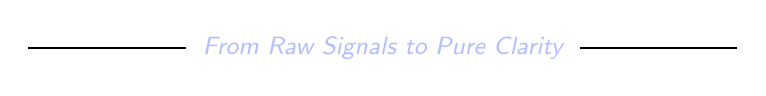
\begin{tikzpicture}
    \draw[left color=transparent, right color=rigelAccent, line width=0.6pt] (-4.5,0) -- (-2.5,0);
    \node[font=\fontsize{9.5}{11}\selectfont\color{rigelAccentLight}\itshape, inner xsep=8pt] at (0,0) 
      {From Raw Signals to Pure Clarity};
    \draw[left color=rigelAccent, right color=transparent, line width=0.6pt] (2.5,0) -- (4.5,0);
  \end{tikzpicture}

  \vspace{5.5mm}

  % 4. Executive Metadata Card (Side-by-Side Dual Pane)
  
\begin{tikzpicture}
    \node[rounded corners=8pt, draw=rigelBorder, line width=0.7pt,
          fill=rigelCard, inner sep=10pt, text width=12.2cm]
    {
      \begin{minipage}[t]{0.54\linewidth}
        {\fontsize{7}{7}\selectfont\bfseries\color{rigelAccent}%
          \tikz\fill[rigelAccent] (0,0.5ex) circle (1.4pt);%
          \hspace{4pt}TEAM ORION \ $\cdot$ \ PRESENTERS}\\[5pt]
        {\fontsize{9.5}{13.5}\selectfont\color{rigelFg}%
          \textbf{MD Mahmudul Hossain Maahi} \hfill \textcolor{rigelMuted2}{\texttt{2305150}}\\[2pt]
          \textbf{Md.\ Shihabul Hasan} \hfill \textcolor{rigelMuted2}{\texttt{2305139}}%
        }
      \end{minipage}%
      \hfill%
      \textcolor{rigelBorder}{\rule[-16pt]{0.5pt}{36pt}}%
      \hfill%
      \begin{minipage}[t]{0.40\linewidth}
        {\fontsize{7}{7}\selectfont\bfseries\color{rigelCyan}%
          \tikz\fill[rigelCyan] (0,0.5ex) circle (1.4pt);%
          \hspace{4pt}PROJECT SUPERVISOR}\\[5pt]
        {\fontsize{9.5}{13.5}\selectfont\color{rigelFg}%
          \textbf{Md.\ Roqunuzzaman Sojib}\\[1.5pt]
          {\fontsize{8}{10}\selectfont\color{rigelMuted2}Department of CSE, BUET}%
        }
      \end{minipage}
    };
  \end{tikzpicture}
  \end{center}
\end{frame}

% ============================================================================
\begin{frame}
  \rigelheader{\rigeltrack{OVERVIEW}}{What We'll Cover}
  \vspace{2mm}
  \begin{itemize}
    \setlength{\itemsep}{5pt}
    \item Motivation \& problem statement
    \item System architecture — how the pieces fit together
    \item A tour of the six DSP workspaces
    \item Live demonstration on real audio
    \item Engineering highlights \& testing
    \item Conclusion \& future work
  \end{itemize}
\end{frame}

% ============================================================================
\begin{frame}
  \rigelheader{\rigeltrack{MOTIVATION}}{Why Rigel?}
  \vspace{3mm}
  \begin{itemize}
    \setlength{\itemsep}{8pt}
    \item Most audio software is a \textbf{black box} — Rigel exposes every transform it performs
    \item Built to make classical Signals \& Systems theory \textbf{tangible}: DFT, STFT, filters, statistical estimation
    \item One connected platform: analyze, filter, denoise, transform, and losslessly encode audio
  \end{itemize}
\end{frame}

% ============================================================================
\begin{frame}
  \rigelheader{\rigeltrack{SYSTEM DESIGN}}{Architecture}
  \vspace{-2mm}
  \begin{center}
  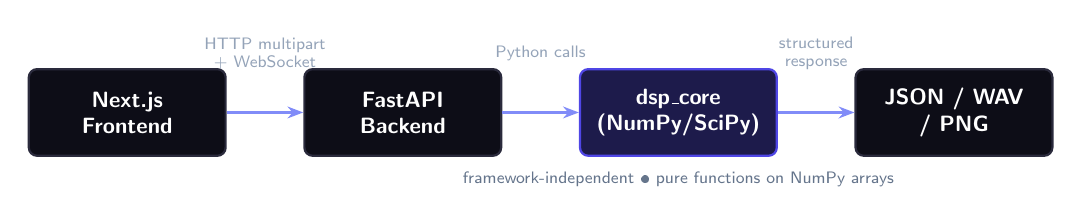
\begin{tikzpicture}[
      box/.style={rounded corners=3pt, draw=rigelBorder, line width=0.8pt,
                  fill=rigelCard, minimum width=2.5cm, minimum height=1.1cm,
                  align=center, font=\fontsize{8.5}{9.5}\selectfont\bfseries\color{rigelFg}},
      lbl/.style={font=\fontsize{6.2}{6.6}\selectfont\color{rigelMuted}, align=center},
      arr/.style={-{Stealth[length=2mm]}, rigelAccent, line width=0.9pt}
    ]
    \node[box] (fe) at (0,0) {Next.js\\Frontend};
    \node[box] (be) at (3.5,0) {FastAPI\\Backend};
    \node[box,fill=rigelPrimary!25!rigelCard,draw=rigelPrimary] (dsp) at (7.0,0) {dsp\_core\\(NumPy/SciPy)};
    \node[box] (out) at (10.5,0) {JSON / WAV\\/ PNG};

    \draw[arr] (fe) -- (be);
    \draw[arr] (be) -- (dsp);
    \draw[arr] (dsp) -- (out);

    \node[lbl] at (1.75,0.75) {HTTP multipart\\ + WebSocket};
    \node[lbl] at (5.25,0.75) {Python calls};
    \node[lbl] at (8.75,0.75) {structured\\response};

    \node[lbl,color=rigelMuted2] at (7.0,-0.85) {framework-independent \textbullet\ pure functions on NumPy arrays};
  \end{tikzpicture}
  \end{center}
  \vspace{0.5mm}
  \footnotesize
  \begin{itemize}\itemsep0pt
    \item \texttt{dsp\_core} never touches HTTP — reusable by any future frontend or a desktop app
    \item Stack: TypeScript, FastAPI, NumPy, SciPy, raw WebSockets for real-time streams
  \end{itemize}
\end{frame}

% ============================================================================
\begin{frame}
  \rigelheader{\rigeltrack{THE PLATFORM}}{Six DSP Workspaces}
  \rigelshot[height=4.3cm]{beamer_assets/02_audio_analysis_1.png}
\end{frame}

% ============================================================================
\begin{frame}
  \rigelheader{\rigeltrack{FOUNDATIONS}}{Audio Analysis}
  \rigelshot[width=0.46\linewidth]{beamer_assets/03_audio_analysis_2_waveform.png}
  \vspace{1.5mm}
  \small
  \begin{itemize}\itemsep2pt
    \item Peak-envelope (min/max) waveform decimation — transients never disappear when zoomed out
    \item Full signal metadata: sample rate, bit depth, duration, channel layout
  \end{itemize}
\end{frame}

% ============================================================================
\begin{frame}
  \rigelheader{\rigeltrack{FREQUENCY DOMAIN}}{Spectrum \& Spectrogram}
  \rigelshot[width=0.48\linewidth]{beamer_assets/04_audio_analysis_3_frequency_spectrum_and_spectogram.png}
  \vspace{1mm}
  \footnotesize
  \begin{itemize}\itemsep1pt
    \item $X[k]=\sum_{n=0}^{N-1} x[n]\,e^{-j2\pi kn/N}$ — an FFT, $O(N\log N)$
    \item STFT: 2048-sample Hann frames, 512-sample hop (75\% overlap)
  \end{itemize}
\end{frame}

% ============================================================================
\begin{frame}
  \rigelheader{\rigeltrack{SPECTRAL LEAKAGE}}{Choice of Window Matters}
  \rigelshot[width=0.66\linewidth]{beamer_assets/05_audio_analysis_4_different_windows.png}
  \vspace{1.5mm}
  \small
  \begin{itemize}\itemsep2pt
    \item Seven windows: Rectangular, Hamming, Hann, Blackman, Kaiser, Bartlett, Welch
    \item Trade-off inherent to every window: main-lobe \textbf{resolution} vs.\ side-lobe \textbf{leakage}
  \end{itemize}
\end{frame}

% ============================================================================
\begin{frame}
  \rigelheader{\rigeltrack{FILTERING}}{Frequency-Selective Filtering}
  \rigelshot[width=0.42\linewidth]{beamer_assets/06_filtering_1_different_types_of_filters.png}
  \vspace{1mm}
  \footnotesize
  \begin{itemize}\itemsep1pt
    \item IIR: Butterworth, Chebyshev I/II, Elliptic, Bessel (stable SOS)
    \item FIR: window method \& Parks--McClellan — zero-phase via \texttt{sosfiltfilt}/\texttt{filtfilt}
  \end{itemize}
\end{frame}

% ============================================================================
\begin{frame}
  \rigelheader{\rigeltrack{FILTERING} \textbullet\ \rigeltrack{RESULT}}{Before \& After}
  \rigelshot[height=4.0cm]{beamer_assets/07_filtering_2_post_filter_application_comparison.png}
  \vspace{1.5mm}
  \small
  \begin{itemize}\itemsep2pt
    \item 1 kHz low-pass: energy above cutoff removed, waveform shape preserved below it
  \end{itemize}
\end{frame}

% ============================================================================
\begin{frame}
  \rigelheader{\rigeltrack{NOISE REMOVAL}}{Statistical Denoising}
  \rigelshot[width=0.42\linewidth]{beamer_assets/08_noise_removal_1.png}
  \vspace{1.5mm}
  \small
  \begin{itemize}\itemsep2pt
    \item Spectral Subtraction $\rightarrow$ Wiener (decision-directed) $\rightarrow$ Log-MMSE $\rightarrow$ IMCRA + OM-LSA
    \item Classical statistical DSP, not deep learning — every gain value is explainable
  \end{itemize}
\end{frame}

% ============================================================================
\begin{frame}
  \rigelheader{\rigeltrack{NOISE REMOVAL} \textbullet\ \rigeltrack{RESULT}}{Denoised Output}
  \rigelshot[height=4.0cm]{beamer_assets/09_noise_noise_removal_2_post_denoising_comparison.png}
  \vspace{1.5mm}
  \small
  \begin{itemize}\itemsep2pt
    \item Broadband noise floor suppressed while speech harmonics are preserved
  \end{itemize}
\end{frame}

% ============================================================================
\begin{frame}
  \rigelheader{\rigeltrack{VOICE ACTIVITY DETECTION}}{Real-Time Speech Detection}
  \rigelshot[height=3.4cm]{beamer_assets/11_vad_2_demonstration.png}
  \vspace{1.5mm}
  \small
  \begin{itemize}\itemsep2pt
    \item Silero \& TEN VAD — hot-swappable engines, same session
    \item Raw Float32 PCM streamed over a binary WebSocket, decision per chunk
  \end{itemize}
\end{frame}

% ============================================================================
\begin{frame}
  \rigelheader{\rigeltrack{VOICE LABORATORY}}{Modular Effect Chain}
  \rigelshot[height=3.4cm]{beamer_assets/15_voice_lab_4_effect_chain.png}
  \vspace{1.5mm}
  \small
  \begin{itemize}\itemsep2pt
    \item Deterministic chain: Gain $\to$ Speed $\to$ Time-Stretch $\to$ Pitch Shift $\to$ Effect
    \item 8 effects: Gain, Pitch Shift, Speed, Time Stretch, Echo/Delay, Reverb, Chorus, Distortion
  \end{itemize}
\end{frame}

% ============================================================================
\begin{frame}
  \rigelheader{\rigeltrack{VOICE LABORATORY}}{Live Voice Measurement}
  \rigelshot[width=0.48\linewidth]{beamer_assets/13_voice_lab_2_live_voice_measurement.png}
  \vspace{1.5mm}
  \small
  \begin{itemize}\itemsep2pt
    \item YIN pitch estimation \& RMS loudness, computed per streamed chunk
    \item Sample rate negotiated client $\to$ server over a JSON WebSocket handshake
  \end{itemize}
\end{frame}

% ============================================================================
\begin{frame}
  \rigelheader{\rigeltrack{VOICE LABORATORY}}{Session Analytics}
  \rigelshot[width=0.48\linewidth]{beamer_assets/14_voice_lab_3_session_stats.png}
  \vspace{1.5mm}
  \small
  \begin{itemize}\itemsep2pt
    \item Peak / RMS loudness, average pitch, pitch range, \% voiced frames
    \item BPM shown only when statistically reliable — never a fabricated number
  \end{itemize}
\end{frame}

% ============================================================================
\begin{frame}
  \rigelheader{\rigeltrack{AUDIO} $\leftrightarrow$ \rigeltrack{IMAGE}}{Encoding Audio as a Data Image}
  \rigelshot[height=3.4cm]{beamer_assets/18_audio_to_image_2_encoded_audio.png}
  \vspace{1.5mm}
  \small
  \begin{itemize}\itemsep2pt
    \item PCM $\to$ FLAC compression $\to$ CRC32-checksummed \texttt{RGL1} packet $\to$ PNG pixels
    \item A literal data container, not steganography — every pixel is payload
  \end{itemize}
\end{frame}

% ============================================================================
\begin{frame}
  \rigelheader{\rigeltrack{AUDIO} $\leftrightarrow$ \rigeltrack{IMAGE} \textbullet\ \rigeltrack{RESULT}}{Recovering Audio, Bit-Exact}
  \rigelshot[height=3.4cm]{beamer_assets/19_audio_to_image_3_decoded_audio.png}
  \vspace{1.5mm}
  \small
  \begin{itemize}\itemsep2pt
    \item CRC32-validated on decode — a corrupted image is rejected, never silently guessed
  \end{itemize}
\end{frame}

% ============================================================================
\begin{frame}[plain]
  \begin{center}
  \vspace{18mm}
  {\fontsize{10}{10}\selectfont\bfseries\color{rigelAccent}\addfontfeature{LetterSpace=140} DEMONSTRATION}\\[6mm]
  {\fontsize{36}{36}\selectfont\bfseries\color{rigelFg} Live Demo}\\[7mm]
  {\fontsize{10}{14}\selectfont\ttfamily\color{rigelMuted} noise\_mono.wav $\rightarrow$ Analysis $\rightarrow$ Denoising $\rightarrow$ Audio$\leftrightarrow$Image}
  \end{center}
\end{frame}

% ============================================================================
\begin{frame}
  \rigelheader{\rigeltrack{UNDER THE HOOD}}{Engineering \& Testing}
  \vspace{2mm}
  \begin{itemize}
    \setlength{\itemsep}{7pt}
    \item \texttt{dsp\_core}: pure NumPy/SciPy, zero framework coupling, fully unit-testable
    \item 480+ backend \texttt{pytest} cases spanning all six modules
    \item Real-time paths: binary WebSocket streaming for VAD and live pitch/RMS
    \item Zero-phase filtering, CRC32-verified codecs, strict NaN/Inf rejection in effects
  \end{itemize}
\end{frame}

% ============================================================================
\begin{frame}
  \rigelheader{\rigeltrack{WRAP-UP}}{Conclusion \& Future Work}
  \vspace{4mm}
  \begin{itemize}
    \setlength{\itemsep}{10pt}
    \item Six complete modules — analysis, filtering, denoising, VAD, voice effects, audio-image codec
    \item A DSP laboratory built to teach, not just to process
    \item Future Plans: a desktop application, active noise cancellation, learned models
  \end{itemize}
\end{frame}

% ============================================================================
% CLOSING SLIDE
% ============================================================================
\begin{frame}[plain]
  \begin{center}

  % Project Logo
  \includegraphics[height=1.4cm,keepaspectratio]{logo.png}\\[4mm]

  % Subtitle / Branding
  {\fontsize{25}{25}\selectfont\color{rigelAccentLight}\rivagefont Rigel}\\[3mm]

  % Primary Heading
  {\fontsize{34}{36}\selectfont\bfseries\color{rigelFg} Thank You}\\[2mm]
  {\fontsize{12}{12}\selectfont\color{rigelMuted}\itshape Questions \& Discussion}

  \end{center}
\end{frame}

\end{document}
